\section{Opis ogólny}

\subsection{Perspektywa produktu}
System SWPFK ma na celu zastąpienie istniejącego systemu, który jest już przestarzały oraz nie spełnia wymagań firmy kurierskiej. Będzie on funkcjonował jako niezależne oprogramowanie wspomagające szereg procesów związanych z usługami dostarczanymi przez firmę.

System będzie udostępniał \textbf{klientom firmy} interfejs za pomocą, którego będą mogli zamówić odpowiednie usługi oraz uzyskać niezbędne informacje. Interfejs ten powinien być oparty na technologii zapewniającej szeroką dostępność dla klientów firmy.

\textbf{Kurierom} system będzie dostarczał mobilnego rozwiązania wspomagającego proces odbioru i doręczenia paczek. Rozwiązanie to będzie zbudowane w oparciu o urządzenia mobilne zapewniające bezprzewodową łączność z systemem.

\textbf{Pracownikom obsługi klienta} system będzie dawał możliwość dostępu do pełnej historii klienta i informacji o nim. Istotne jest aby wykorzystany interfejs zapewniał wysoką przejrzystość prezentowanych danych.

\textbf{Pracownicy sortowni} będą mieli dostęp do interfejsów zapewniających im pomoc w odpowiednim uszeregowaniu paczek oraz zaplanowaniu trasy doręczenia aby zmaksymalizować efektywność tych procesów. Wspomniany interfejs powinien zapewniać wysoką wydajność oraz przyjazną wizualizację wyników algorytmu.

System będzie również udostępniał interfejsy umożliwiające integrację z \textbf{systemami zewnętrznych firm} transportowych w celu korzystania z ich usług z poziomu SWPFK.

Rysunek \ref{diag:perspektywa} przedstawia diagram kontekstu dla SWPFK. Zawiera on podstawowych aktorów prowadzących interakcję z systemem oraz podstawowe informacje jakie będą z~nim wymieniać.

\begin{figure}[ht]
	\centering
	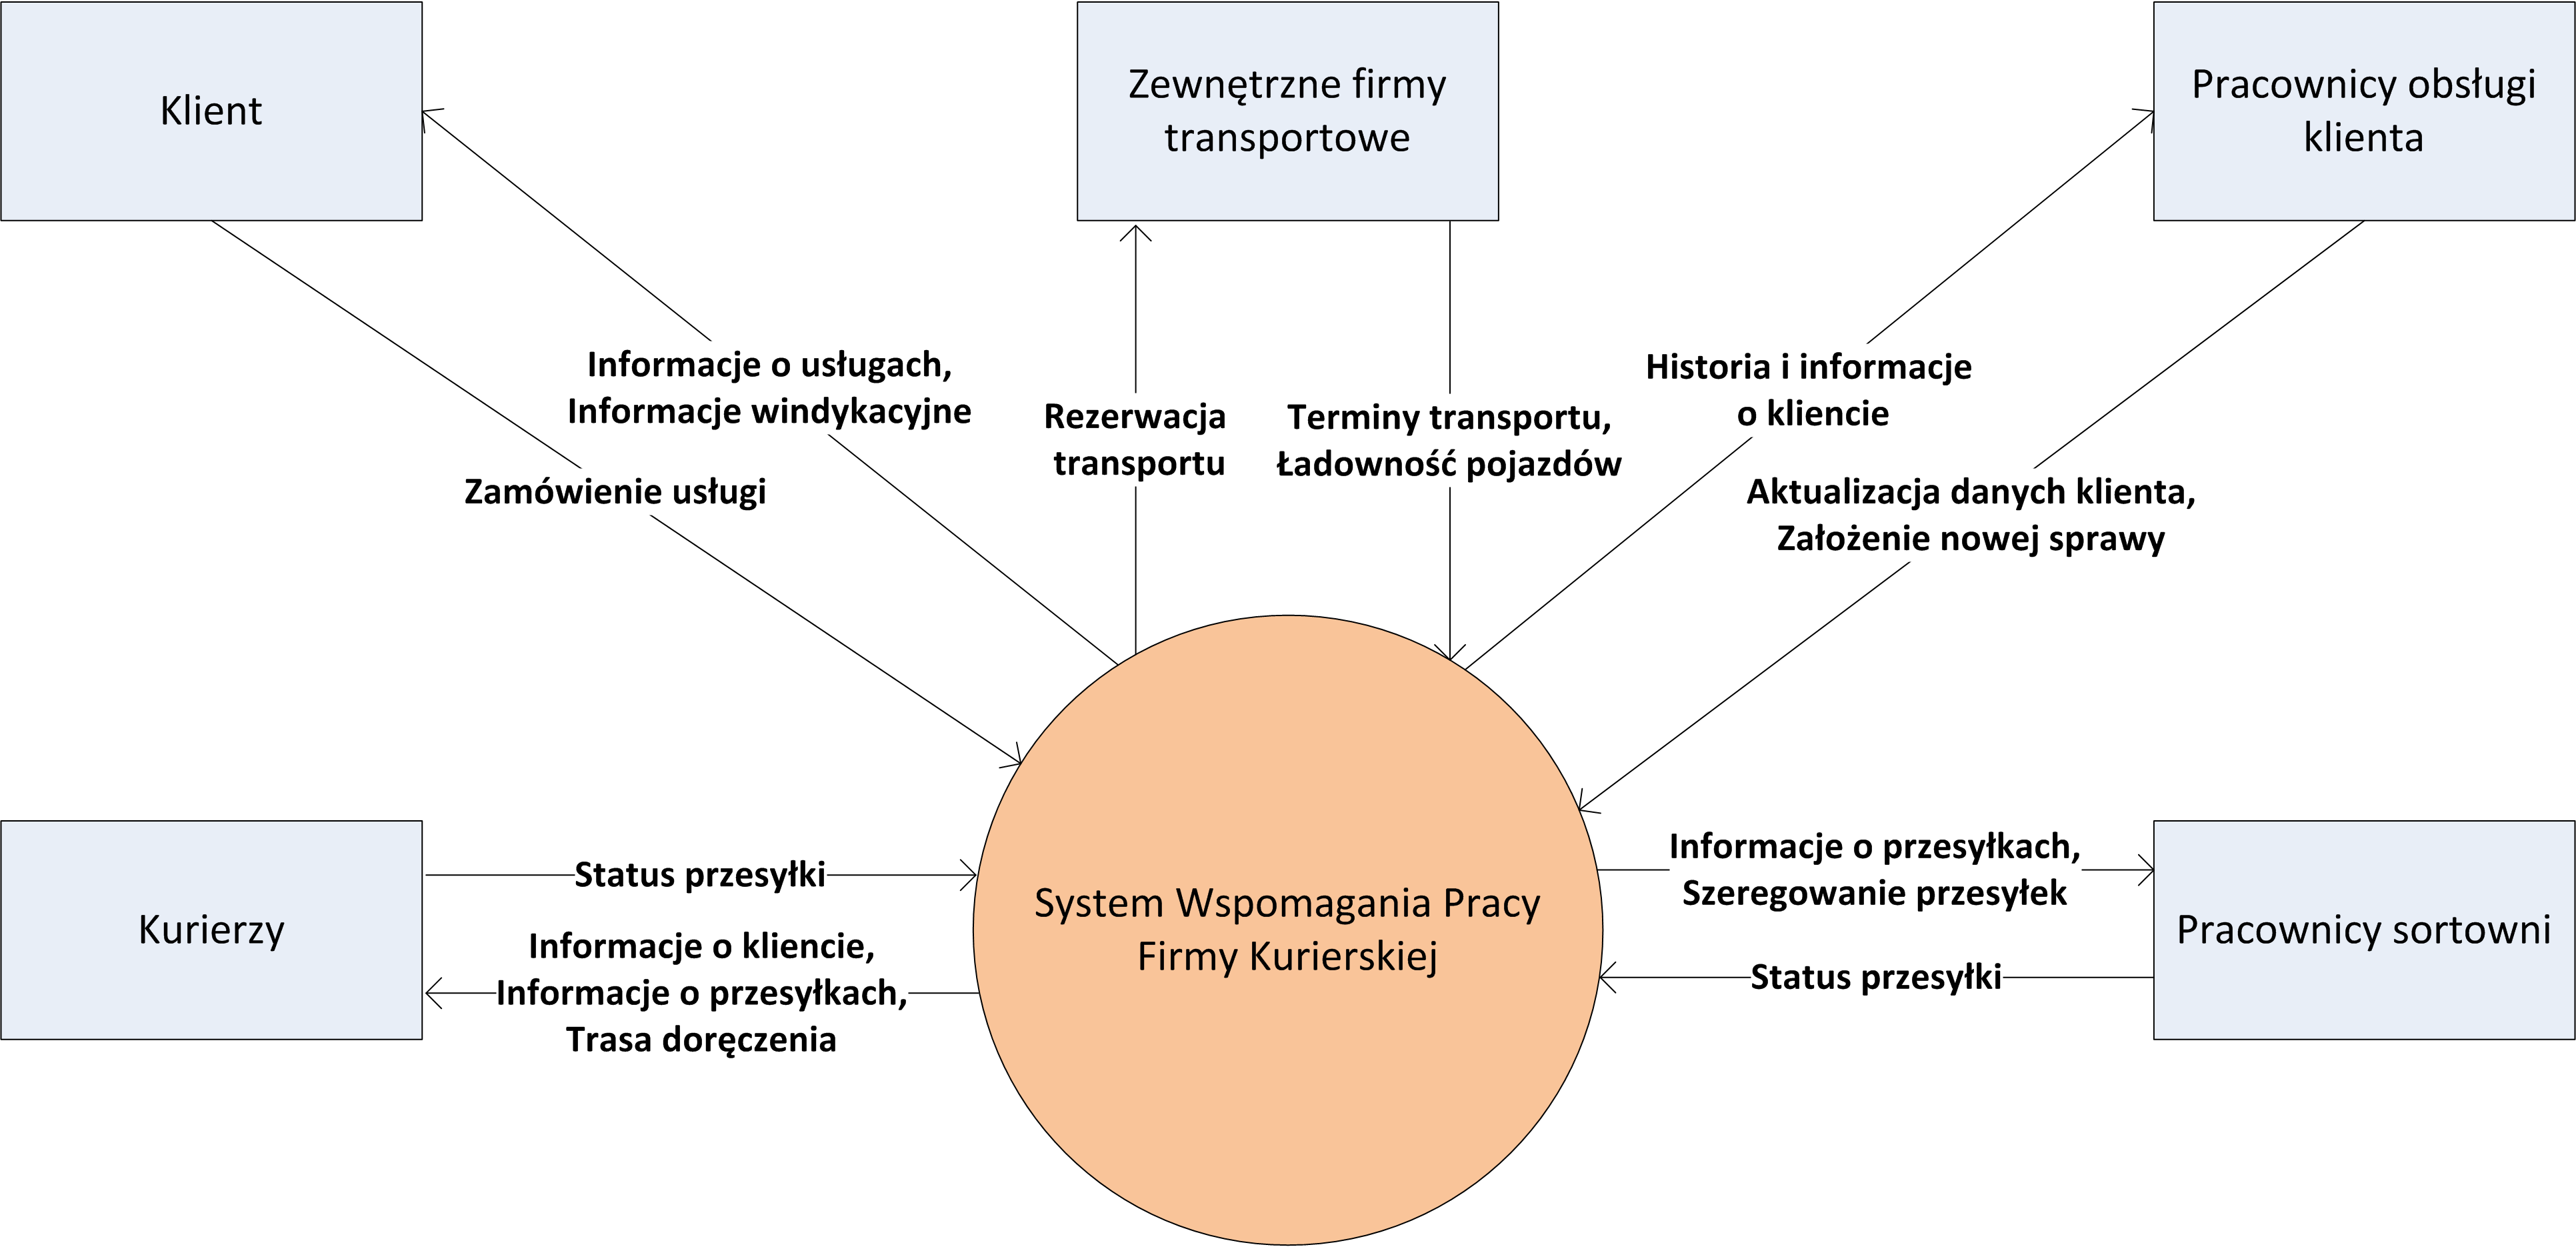
\includegraphics[width=\textwidth]{img/perspektywa}
	\caption{Diagram kontekstu dla SWPFK.}
	\label{diag:perspektywa}
\end{figure}

\subsection{Funkcje produktu}
Podstawową funkcją SWPFK będzie możliwość rejestracji przesyłki w systemie oraz śledzenie jej drogi od momentu nadania do doręczenia. Ponadto pozwoli on na odpowiednie zoptymalizowanie transportu paczek oraz wyznaczenie najlepszej drogi ich doręczenia do adresata.

System będzie zapewniał klientom firmy kurierskiej możliwość stałego dostępu do szczegółowych informacji na temat usług świadczonych przez firmę. SWPFK będzie również udostępniał możliwość zamówienia dowolnej usługi za pomocą odpowiednich interfejsów, skorzystania z pomocy obsługi klienta oraz rejestracji klienta w systemie.

Pracownicy obsługi klienta będą używać SWPFK w celu:
\begin{itemize}
\item obsługi klientów w POK;
\item dostępu do przekrojowej informacji o kliencie, która będzie zawierała m. in. jego pełną historię;
\item obsługi klientów kanałem online.
\end{itemize}

System będzie również umożliwiał zamówienie usługi transportu w zewnętrznej firmie transportowej oraz obsługę windykacji w szczególności klientów masowych.

\subsection{Ograniczenia}

\subsubsection{Zgodność z aktami prawnymi}
SWPFK musi być zgodny z rozporządzeniami oraz ustawami wymieniowymi w rozdziale \ref{subsec:Literatura} w punktach 1, 2 oraz 3.

\subsubsection{Zgodność ze standardami i normami}
Dokumentacja użytkownika musi być zgodna ze standardem IEEE 1063-2001 (punkt 4 w rozdziale \ref{subsec:Literatura}).

\subsubsection{System zarządzania bazą danych}
Firma Kurierska posiada 4 licencje na bazę danych firmy Oracle w wersji 10g z możliwością aktualizacji do wersji 11g. Licencje są w wersji Enterprise Edition oraz typu procesorowego co pozwala na użytkowanie bazy przez wielu użytkowników. Do licencji zostało również wykupione wsparcie na wypadek wystąpienia problemów w obsłudze bazy danych.

Ze względu na posiadane licencje SWPFK powinien być zbudowany w oparciu o bazę danych firmy Oracle. SWPFK będzie agregował duże ilości danych dotychczas rozproszonych po odseparowanych systemach co może skutkować koniecznością dokupienia większej ilości licencji, aby móc zainstalować system na sprzęcie o większej mocy obliczeniowej.

Wykorzystanie posiadanych licencji pozwoli na obniżenie kosztów systemu oraz zaangażowanie dotychczas zdobytego doświadczenia w obsłudze baz danych Oracle.

\subsubsection{Ograniczenia sprzętowe}
%TODO

\subsubsection{Protokoły komunikacyjne}
Komunikacja pomiędzy modułem serwerowym systemu a aplikacjami klienckimi oraz mobilnymi będzie się odbywać za pomocą kanału komunikacyjnego wspierającego szyfrowanie protokołem TLS w wersji co najmniej 1.1. Minimalna długość klucza służącego do zabezpieczenia połączenia musi wynosić 128 bitów.

SWPFK będzie udostępniał interfejs internetowy który będzie używał do komunikacji protokołu HTTP w przypadku informacji publicznych oraz HTTPS w przypadku informacji poufnych.

\subsubsection{Instalacja oprogramowania}
%TODO

\subsubsection{Interfejsy programistyczne}
SWPFK powinien posiadać elastyczny interfejs (API) pozwalający w przyszłości na łatwą integrację z systemami innych zewnętrznych firm transportowych.

\subsection{Dokumentacja użytkownika}
%TODO

\subsection{Założenia i zależności}
Zakłada się, że użytkownik interfejsu internetowego SWPFK będzie korzystał z jednej z poniższych przeglądarek internetowych:
\begin{enumerate}
\item Internet Explorer 10, 11;
\item Mozilla Firefox w wersji co najmniej 28;
\item Google Chrome w wersji 35 lub wyższej;
\item Apple Safari w wersji co najmniej 5.
\end{enumerate}

Zakłada się, że użytkownicy aplikacji klienckiej na komputer PC będą korzystać z systemu Microsoft Windows Vista lub jego nowszej wersji. Ponadto użytkownicy będą mieli zainstalowane oprogramowanie Microsoft .NET Framework w wersji co najmniej 3.5.